
%(BEGIN_QUESTION)
% Copyright 2014, Tony R. Kuphaldt, released under the Creative Commons Attribution License (v 1.0)
% This means you may do almost anything with this work of mine, so long as you give me proper credit

This inductive liquid level relay produces 800 volts between the sensing probes when no contact is made with the liquid, from a 120 volt AC power source:

$$\includegraphics[width=15.5cm]{i00035x01.eps}$$

Assuming 200 turns of wire in its primary winding, calculate the following parameters.  Assume for the sake of simplicity that the relay's armature has not yet ``picked up'' when the liquid first contacts the probe tips:

\vskip 10pt

\begin{itemize}
\item{} Number of turns in the secondary winding = \underbar{\hskip 50pt}
\vskip 10pt 
\item{} Primary winding current when liquid $R$ is 20,000 $\Omega$ = \underbar{\hskip 50pt}
\vskip 10pt 
\item{} Secondary winding current when liquid $R$ is 20,000 $\Omega$ = \underbar{\hskip 50pt}
\end{itemize}

\vskip 10pt

Also, explain why it is important to know that the armature is still in its ``resting'' position for the sake of these calculations.

\vfil 

\underbar{file i00035}
\eject
%(END_QUESTION)





%(BEGIN_ANSWER)

This is a graded question -- no answers or hints given!

%(END_ANSWER)





%(BEGIN_NOTES)

The number of turns in the secondary winding is that necessary to produce a ratio (with the 200 turns in the primary winding) capable of stepping up 120 volts to 800 volts:

$${800 \hbox{ V} \over 120 \hbox{ V} } = {x \over 200 \hbox{ turns}}$$

$$x = 200 \hbox{ turns} \left( 800 \hbox{ V} \over 120 \hbox{ V} \right)$$

$$x = 1333 \hbox{ turns}$$

\vskip 10pt

Secondary winding current is simply determined by applying Ohm's Law, taking 800 volts and dividing by the resistance of the liquid between the probe contacts:

$$I = {V \over R} = {800 \hbox{ V} \over 20000 \> \Omega} = 40 \hbox{ mA}$$

\vskip 10pt

Primary winding current must be greater than this, since primary winding voltage is {\it less} than secondary winding voltage and power ($P = IV$) must be the same on both sides of the transformer.  We may therefore take the voltage ratio given to us (800:120) and use this to calculate primary winding current from secondary winding current:

$$I_{primary} = 40 \hbox{ mA} \left( 800 \over 120 \right) = 266.7 \hbox{ mA}$$

\vskip 10pt

It is important to know that the armature is in its resting position in these calculations because when it is such the inductive level relay acts like a simple step-up transformer.  Once the armature picks up, a new magnetic circuit is formed in the relay core which shunts much of the primary winding's magnetic flux away from the secondary winding.  When that happens, the secondary winding outputs much less than 800 volts, and all the current values will become diminished as well!

%INDEX% Switch, level: liquid conductivity

%(END_NOTES)


